\documentclass[landscape,final,a0paper]{baposter}


\tracingstats=2

\usepackage{calc}
\usepackage{graphicx}
\usepackage{amsmath}
\usepackage{amssymb}
\usepackage{relsize}
\usepackage{multirow}
\usepackage{bm}

\usepackage{graphicx}
\usepackage{multicol}

\usepackage{pgfbaselayers}
\pgfdeclarelayer{background}
\pgfdeclarelayer{foreground}
\pgfsetlayers{background,main,foreground}

\usepackage{times}
\usepackage{helvet}
\usepackage{palatino}
\usepackage[utf8x]{inputenc}
\usepackage{amssymb, upgreek}

\usepackage{color}
\definecolor{keywordcolor}{rgb}{0.7, 0.1, 0.1}   % red
\definecolor{commentcolor}{rgb}{0.4, 0.4, 0.4}   % grey
\definecolor{symbolcolor}{rgb}{0.0, 0.1, 0.6}    % blue
\definecolor{sortcolor}{rgb}{0.1, 0.5, 0.1}      % green
\definecolor{errorcolor}{rgb}{1, 0, 0}           % bright red
\definecolor{stringcolor}{rgb}{0.5, 0.3, 0.2}    % brown

\usepackage{listings}
\def\lstlanguagefiles{lstlean.tex}
\lstset{language=lean}

\usepackage{hyperref}

\DeclareUrlCommand\url{\color{magenta}\def\UrlLeft{http://}\urlstyle{tt}}

\newcommand{\captionfont}{\footnotesize}

\selectcolormodel{cmyk}

%\graphicspath{{images/}}

%%%%%%%%%%%%%%%%%%%%%%%%%%%%%%%%%%%%%%%%%%%%%%%%%%%%%%%%%%%%%%%%%%%%%%%%%%%%%%%%
%%%% Some math symbols used in the text
%%%%%%%%%%%%%%%%%%%%%%%%%%%%%%%%%%%%%%%%%%%%%%%%%%%%%%%%%%%%%%%%%%%%%%%%%%%%%%%%
% Format 

\renewcommand{\Pr}{\mbox{P}}
\newcommand{\e}{\mbox{e}}
\newcommand{\dx}{\,\mbox{d}x}

%%%%%%%%%%%%%%%%%%%%%%%%%%%%%%%%%%%%%%%%%%%%%%%%%%%%%%%%%%%%%%%%%%%%%%%%%%%%%%%%
% Multicol Settings
%%%%%%%%%%%%%%%%%%%%%%%%%%%%%%%%%%%%%%%%%%%%%%%%%%%%%%%%%%%%%%%%%%%%%%%%%%%%%%%%
\setlength{\columnsep}{0.7em}
\setlength{\columnseprule}{0mm}


%%%%%%%%%%%%%%%%%%%%%%%%%%%%%%%%%%%%%%%%%%%%%%%%%%%%%%%%%%%%%%%%%%%%%%%%%%%%%%%%
% Save space in lists. Use this after the opening of the list
%%%%%%%%%%%%%%%%%%%%%%%%%%%%%%%%%%%%%%%%%%%%%%%%%%%%%%%%%%%%%%%%%%%%%%%%%%%%%%%%
\newcommand{\compresslist}{%
\setlength{\itemsep}{1pt}%
\setlength{\parskip}{0pt}%
\setlength{\parsep}{0pt}%
}


%%%%%%%%%%%%%%%%%%%%%%%%%%%%%%%%%%%%%%%%%%%%%%%%%%%%%%%%%%%%%%%%%%%%%%%%%%%%%%
%%% Begin of Document
%%%%%%%%%%%%%%%%%%%%%%%%%%%%%%%%%%%%%%%%%%%%%%%%%%%%%%%%%%%%%%%%%%%%%%%%%%%%%%

\begin{document}

%%%%%%%%%%%%%%%%%%%%%%%%%%%%%%%%%%%%%%%%%%%%%%%%%%%%%%%%%%%%%%%%%%%%%%%%%%%%%%
%%% Here starts the poster
%%%---------------------------------------------------------------------------
%%% Format it to your taste with the options
%%%%%%%%%%%%%%%%%%%%%%%%%%%%%%%%%%%%%%%%%%%%%%%%%%%%%%%%%%%%%%%%%%%%%%%%%%%%%%
% Define some colors
\definecolor{silver}{cmyk}{0,0,0,0.3}
\definecolor{yellow}{cmyk}{0,0,0.9,0.0}
\definecolor{reddishyellow}{cmyk}{0,0.22,1.0,0.0}
\definecolor{black}{cmyk}{0,0,0.0,1.0}
\definecolor{darkYellow}{cmyk}{0,0,1.0,0.5}
\definecolor{darkSilver}{cmyk}{0,0,0,0.1}
\definecolor{lightyellow}{cmyk}{0,0,0.3,0.0}
\definecolor{lighteryellow}{cmyk}{0,0,0.1,0.0}
\definecolor{lighteryellow}{cmyk}{0,0,0.1,0.0}
\definecolor{lightestyellow}{cmyk}{0,0,0.05,0.0}
\definecolor{cyan}{cmyk}{1,0,0,0}
\definecolor{lightcyan}{cmyk}{0.5,0,0,0}
\definecolor{pastelcyan}{cmyk}{0.25,0,0,0}
\definecolor{magenta}{cmyk}{0,1,0,0}
\definecolor{yellow}{cmyk}{0,0,1,0}
\definecolor{lightyellow}{cmyk}{0,0,0.5,0}
\definecolor{pastelyellow}{cmyk}{0,0,0.25,0}
\definecolor{black}{cmyk}{0,0,0,1}
\definecolor{darkgray}{cmyk}{0,0,0,0.75}
\definecolor{gray}{cmyk}{0,0,0,0.5}
\definecolor{lightgray}{cmyk}{0,0,0,0.25}
\definecolor{white}{cmyk}{0,0,0,0}
\definecolor{red}{cmyk}{0,1,1,0}
\definecolor{orange}{cmyk}{0,0.5,1,0}
\definecolor{scarlet}{cmyk}{0,1,0.5,0}
\definecolor{brown}{cmyk}{0.5,0.75,1,0}
\definecolor{camel}{cmyk}{0.25,0.375,0.5,0}
\definecolor{cream}{cmyk}{0,0.2,0.3,0}
\definecolor{green}{cmyk}{1,0,1,0}
\definecolor{lightgreen}{cmyk}{0.5,0,0.5,0}
\definecolor{pastelgreen}{cmyk}{0.25,0,0.25,0}
\definecolor{mossgreen}{cmyk}{0.64,0.4,1,0}
\definecolor{yellowgreen}{cmyk}{0.5,0,1,0}
\definecolor{skyblue}{cmyk}{0.4,0.16,0,0}
\definecolor{royal}{cmyk}{1.0,0.5,0,0}
\definecolor{navyblue}{cmyk}{0.9,0.75,0.5,0}
\definecolor{lightnavy}{cmyk}{0.4,0.3,0.2,0}
\definecolor{blue}{cmyk}{1,1,0,0}
\definecolor{lightblue}{cmyk}{0.5,0.5,0,0}
\definecolor{pastelblue}{cmyk}{0.25,0.25,0,0}
\definecolor{lightpastelblue}{cmyk}{0.15,0.15,0,0}
\definecolor{lightestpastelblue}{cmyk}{0.05,0.05,0,0}
\definecolor{lavender}{cmyk}{0.25,0.25,0,0}
\definecolor{violet}{cmyk}{0.75,1,0.25,0}
\definecolor{purple}{cmyk}{0.5,1,0.5,0}
\definecolor{lightpurple}{cmyk}{0.25,0.5,0.25,0}
\definecolor{pink}{cmyk}{0,0.5,0,0}


%%

\typeout{Poster Starts}
%\background{
  %\begin{tikzpicture}[remember picture,overlay]%
  %  \draw (current page.north west)+(-2em,-2em) node[anchor=north west] %{\hspace{-2em}\includegraphics[height=1.1\textheight]{silhouettes_background}};
 % \end{tikzpicture}%
%}




\newlength{\leftimgwidth}
\begin{poster}%
  % Poster Options, such as colours etc
  {
  % Show grid to help with alignment
  grid=false,
 % Column spacing
  colspacing=0.5em,
 % Color style
 % bgColorOne=pastelblue,
 %bgColorTwo=lightpastelblue,
  bgColorOne=white,
  bgColorTwo=white,
  borderColor=navyblue,
  headerColorOne=lightnavy,
  headerColorTwo=purple,
  headerFontColor=black,
 % boxColorOne=lightpastelblue,
 % boxColorTwo=lightestpastelblue,
 boxColorOne=white,
 boxColorTwo=white,
 % Format of textbox
  textborder=roundedleft,
% textborder=rectangle,
% Format of text header
  eyecatcher=false,
  headerborder=open,
  headerheight=0.08\textheight,
  headershape=roundedright,
  headershade=plain,
  headerfont=\Large\textsf, %Sans Serif
  boxshade=plain,
%  background=shade-tb,
 % background=plain,
  background=none,
  linewidth=2pt
  }
  % Eye Catcher
  {} % select eyecatcher=false above if not required. If no eye catcher is present, the title is left aligned.
  % Title
  {\sf %Sans Serif
  %\bf% Serif
  \vspace*{5mm}
  \hspace*{2mm} The Formalisation and Applications of the Stone-Weierstrass Theorem}
  % Authors
  {\hspace*{4.5mm} Kexing Ying \\
   \hspace*{4.5mm} \url{imperial.cloud.panopto.eu/Panopto/Pages/Viewer.aspx?id=2d5eb25d-c698-44f3-a1a1-abd700fe1f51}
  }
  % University logo
  { % The makebox allows the title to flow into the logo
    \makebox[8em][r]{%
        \begin{minipage}{16em}
				\hfill 
\includegraphics[height=3em]{imperial.pdf}
				\end{minipage}
      
    }
  }

  \tikzstyle{light shaded}=[top color=baposterBGtwo!30!white,bottom color=baposterBGone!30!white,shading=axis,shading angle=30]

  % Width of left inset image
     \setlength{\leftimgwidth}{0.78em+8.0em}

%%%%%%%%%%%%%%%%%%%%%%%%%%%%%%%%%%%%%%%%%%%%%%%%%%%%%%%%%%%%%%%%%%%%%%%%%%%%%%
%%% Now define the boxes that make up the poster
%%%---------------------------------------------------------------------------
%%% Each box has a name and can be placed absolutely or relatively.
%%% The only inconvenience is that you can only specify a relative position 
%%% towards an already declared box. So if you have a box attached to the 
%%% bottom, one to the top and a third one which should be in between, you 
%%% have to specify the top and bottom boxes before you specify the middle 
%%% box.
%%%%%%%%%%%%%%%%%%%%%%%%%%%%%%%%%%%%%%%%%%%%%%%%%%%%%%%%%%%%%%%%%%%%%%%%%%%%%%
    %
    % A coloured circle useful as a bullet with an adjustably strong filling
\newcommand{\colouredcircle}[1]{%
      \tikz{\useasboundingbox (-0.2em,-0.32em) rectangle(0.2em,0.32em); \draw[draw=black,fill=baposterBGone!80!black!#1!white,line width=0.03em] (0,0) circle(0.18em);}}

  \headerbox{The Stone-Weierstrass Theorem}{name=stone,column=0,span=1, row=0}{
Let $X$ be a compact metric space and $M$ the set of all continuous function from $X$ to $\mathbb{R}$, then the 
\textit{Stone-Weierstrass theorem} states that, 
\begin{minipage}{0.97\textwidth}
\centering
\noindent\fbox{%
    \parbox{\textwidth}{%
      Given an unital subalgebra of $M$, $M_0$ (i.e. a subset of $M$ that contains 1 and is closed under addition, multiplication and scalar multiplication) that is closed under the lattice operations and separates points, $\bar{M_0} = M$; \cite{gaddy}
    }%
}
\end{minipage}\\
where we define the lattice operations \(\vee, \wedge : (X \to \mathbb{R})^2\to (X \to \mathbb{R}) \) 
such that, for all \(f, g : X \to \mathbb{R}\), where \(f, g\) are continuous functions 
$$
f \vee g = \max\{f, g\}; \hspace{2mm} f \wedge g = \min \{f, g\};
$$
$\bar{M_0}$ the closure of $M_0$ \textit{under uniform convergence to the limit} 
and we say $M_0$ \textit{separates points} if and only if for all distinct $x, y \in X$, there exists some $f \in M_0$ such that $f(x) \neq f(y)$.

\vspace{0.3em}
 }
 
   \headerbox{Lemma: $\left|x\right|$ is in the Closure!}{name=modulus,column=1,span=1, row = 0}{

Let $X_1, \cdots X_n$ be a sequence of i.i.d. Bernoulli random variables with parameter $x$ and let $S_n = \sum_{i= 1}^n X_i$ so $S_n \sim Bin(n, x)$. Then by the \textit{law of the unconscious statistician}, we see, 
$$
\mathbb{E}\left(\left| \alpha \frac{S_n}{n} - \beta \right| \right) = \sum_{k=0}^n \left| \alpha \frac{k}{n} - \beta \right|\text{Pr}\left(S_n = nk\right)
$$ 
\vspace{-3mm}$$
 = \sum_{k=0}^n \left| \alpha \frac{k}{n} - \beta \right| \binom{n}{i} x^i (1 - x)^{n - i} =: P_n(x)
$$
for all $\alpha, \beta \in \mathbb{R}$, $\alpha < \beta$. Let us now define
$$ A_n(\delta) = \left\{\omega : \left| \frac{S_n(\omega)}{n} - x \right| \ge \delta \right\},$$
then, for all $\epsilon > 0$, as $f(x) : [0, 1] \to \mathbb{R} := \left| \alpha x - \beta \right|$ is continuous on the compact interval $[0, 1]$, it is uniformly continuous on the same interval; so there is some $\delta > 0$ such that for all $\left| x - y \right| < \delta$,  $\frac{\epsilon}{2} > \left| f(x) - f(y) \right|$. Now, by LLN, $\text{Pr}(A_n (\delta)) \to 0$, so, choose $N $ such that $\left|\text{Pr}(A_N(\delta)) \right| < 1/2$, then
\begin{align*}
\frac{\epsilon}{2} & > \mathbb{E} \left[ \mathbf{1}_{(A_N)^c}\left| f(x) - f \left(\frac{S_N}{N}\right) \right| \mid A_N(\delta)^c \right] \\
& \ge \left| f(x) - \mathbb{E} \left[f \left(\frac{S_N}{N}\right) \right] \right| \text{Pr}((A_N(\delta))^c).
\end{align*}
Now as $\mathbb{E} \left[f \left(\frac{S_N}{N}\right) \right] = P_N(x)$, we have $\epsilon/ 2 > \left|f(x) - P_N(x)\right| (1 - \text{Pr}(A_N(\delta))) > \left|f(x) - P_N(x)\right|/2$, so $P_n(x) \to f(x) = \left| \alpha x - \beta \right|$ uniformly for $x\in [0,1]$ and $P_n(\frac{x + \beta}{\alpha}) \to \left| x \right|$ uniformly for all $x \in [\alpha, \beta]$.


\vspace{0.3em}
 }

%%%%%%%%%%%%%%%%%%%%%%%%%%%%%%%%%%%%%%%%%%%%%%%%%%%%%%%%%%%%%%%%%%%%%%%%%%%%%%
  \headerbox{Application: Weierstrass Theorem}{name=approx,column=0,span=1, below=stone}{
	
The Weierstrass approximation theorem states 
\begin{minipage}{0.97\textwidth}
\centering
\noindent\fbox{%
    \parbox{\textwidth}{%
 Let $f$ be a real continuous function on a closed interval $[\alpha, \beta]$. Then for all $\epsilon > 0$, there exists a polynomial 
$P_n$ such that 
$$\sup_{x \in [\alpha, \beta]} \left| f(x) - P_n(x) \right| < \epsilon. $$
    }%
}
\end{minipage}\\ 

\vspace{2mm}
By section \textit{Lemma: $\left|x\right|$ is in the Closure!}, the sequence of polynomial $P_n(x) \to \left| x \right|$ uniformly where,
$$
P_n(x) := \sum_{k=0}^n \left| \alpha \frac{k}{n} - \beta \right| \binom{n}{i} x^i (1 - x)^{n - i}
$$
 Now, as 
$$f \vee g = \frac{1}{2}(f + g + \left| f - g \right|);$$
$$f \wedge g = \frac{1}{2}(f + g - \left| f - g \right|),$$
we see $\bar{\mathcal{P}}$ (the closure of polynomials under uniform convergence) is closed under the lattice operations. Thus, as $\bar{\mathcal{P}}$ form an unital subalgebra of all real to real functions, (as it contains 1, closed under addition, multiplication and scalar multiplication), and as $\bar{\mathcal{P}}$ separates points trivially, $\bar{\bar{\mathcal{P}}} = \bar{\mathcal{P}} = [\alpha, \beta]^\mathbb{R}$ for all $\alpha, \beta \in \mathbb{R}, \alpha < \beta$ as required!
  \vspace{0.2em}
  }

 \headerbox{Application: Trig. Polynomials}{name=trig,column=1,span=1,below=modulus}{
 
Another set of functions that are interesting are the trigonometric polynomials $\mathcal{T}$.
As any constant is a trigonometric polynomial, $1 \in \mathcal{T}$ while $\mathcal{T}$ is trivially closed under addition and scalar multiplication. Thus, by considering the identity
$$
\sin(n x) \cos(k x) = \frac{1}{2}(\cos(n-k)x - \cos(n+k)x),
$$
and similarly the identities of $\sin(nx)\sin(kx)$ and $\cos(nx)\cos(kx)$, $\mathcal{T}$ is closed under multiplication. Thus 
$\mathcal{T}$ form an unital subalgebra of continuous functions on \([-\pi, \pi]\),
and by considering the Fourier series of $\left| x \right|$,
$\bar{\mathcal{T}}$ is closed under lattice operations and hence, by Stone-Weierstrass, 
$\bar{\bar{\mathcal{T}}} = \bar{\mathcal{T}} = [-\pi, \pi]^\mathbb{R}$.

  \vspace{0.2em}
  }

 \headerbox{Further Discussion \& Interpolation}{name=inter,column=3,span=1,row=0}{
The Stone-Weierstrass theorem proved the density of polynomial functions, but does not provide a construction. We can achieve this using the Bernstein polynomials.
Consider the approximation of $x^2$ for $x \in [0, 1]$ using Bernstein polynomials,
$$B_n(x)=\frac{1}{n} x + \frac{n-1}{n} x^2.$$
By using calculus, we find $\sup_{x\in[0, 1]} \left|x^2 - B_n(x) \right| = (4n)^{-1}$; much worse than just using $x^2$ as its own approximation.
\begin{center}
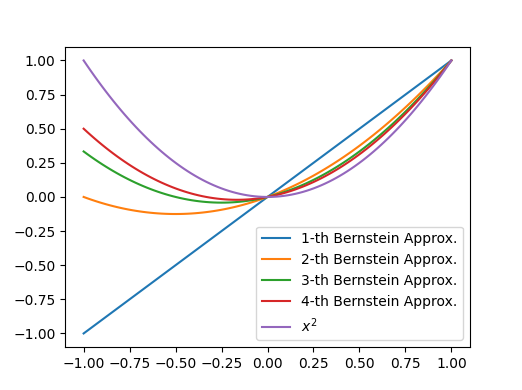
\includegraphics[scale = 0.4]{x_squared}
\end{center}

\vspace{-2mm}
Consider instead the Lagrange interpolation \cite{humph}.

Given $(x_0, y_0), \cdots, (x_n, y_n)$ be $n$ distinct points, we want polynomial $L_n(x) = \sum_{i=0}^n a_ix^i$, $L_n(x_i) = y_i$  $\implies V[a_i] = [y_i]$ where $V$ is the Vandermonde matrix such that $V_{i,j} = x_{i-1}^{j-1}$. As $V_{i,j}$ is invertible by the Vandermonde determinant, we found an unique coefficient vector interpolating these points.


\vspace{2mm}
Let $f : [a, b] \to \mathbb{R}$ be a continuous, we can approximate $f$ using the polynomial that interpolates the set of equidistant points from $a$ to $b$. With Python, we find that for $n = 3$ for $x^2$ on $[0, 1]$, this method results in a polynomial approximation of $L_3(x) = x^2$.

\vspace{2mm}
However, $\lVert f - P_n \rVert_\infty$ does not necessarily tends to 0 exemplified by \textit{Runge's function}. To mitigate this, one can instead use \textit{Spline interpolation} however this results in an approximant that is a piecewise polynomial instead of just a polynomial.

  \vspace{0.2em}
  }  

 %%%%%%%%%%%%%%%%%%%%%%%%%%%%%%%%%%%%%%%%%%%%%%%%%%%%%%%%%%%%%%%%%%%%%%%%%%%%%
\headerbox{Proof Outline of Stone-Weierstrass}{name=form,column=2,span=1,row=0}{
{\bf Lemma 1.} For all $f \in M$, $f$ is in $\bar{M_0}$ if and only if for all $x, y \in X$, $\epsilon > 0$, there 
exists $g \in M_0$ such that $\left| f(x) - g(x) \right| < \epsilon$ and $\left| f(y) - g(y) \right| < \epsilon$.

\textit{Proof.} The forward direction is by definition so we consider the reverse. Suppose for all $x, y \in X$, $\epsilon > 0$, there 
exists $g \in M_0$ such that $\left| f(x) - g(x) \right| < \epsilon$ and $\left| f(y) - g(y) \right| < \epsilon$ $(*)$. Let us fix $x$ and $\epsilon$ and define the mapping
$$S(y) := \{z \in X \mid f(z) - g_y(z) < \epsilon \},$$
where $g_y$ was chosen such that $\left| f(x) - g_y(x) \right| < \epsilon$ and $\left| f(y) - g_y(y) \right| < \epsilon$ which existence is guaranteed by $(*)$.

Then for all $y \in X$, $y \in S(y)$ so $\bigcup_{y\in X} S(y) = X$. But as $X$ is compact, $\bigcup_{y\in X} S(y)$ admits a finite subcover; 
so, there exists a finite index set $I$ such that $\bigcup_{i\in I} S(y_i) = X$. Thus, by letting $p_x = \bigvee_{i \in I} g_{y_i}$, we have constructed 
a function $p_x \in  \bar{M_0}$ such that 
$$
p_x(z) \ge g_{y_i}(z) > f(z) - \epsilon \hspace{1mm} \text{and} \hspace{1mm} p_x(x) < f(x) + \epsilon
$$
for all $z \in X$ and $i \in I$	.

Now, by defining a similar mapping, $T$,  
$$T := \{z \in X \mid p_x(z) < f(z) + \epsilon \},$$
we again create a finite subcover of $X$ and thus can create the required function with $\bigwedge_{j \in J}p_{x_j}$ where $J$ 
is the index set such that $\bigcup_{j\in J} T(x_j) = X$.

\vspace{2mm}
{\bf Lemma 2.} Given $S$, a subalgebra of $\mathbb{R}^2$, $S$ must be $\{(0,0)\}$, 
$\{(x, 0) \mid x \in \mathbb{R} \}$,
$\{(0. y) \mid y \in \mathbb{R} \}$, 
$\{(z, z) \mid z \in \mathbb{R} \}$, or
$\mathbb{R}^2$ itself.

\textit{Lemma 2} was proved by evoking the law of the excluded middle on different propositions.

\vspace{2mm}
Given $x, y \in X$, define the boundary points of $M_0$ to be $\{(f(x), f(y)) \mid f \in M_0 \}$.
Let $M_0$, $M_1$ be closed subalgebras of $M$ under lattice operations,
by lemma 1, it is deduced $\bar{M_0} = \bar{M_1}$ iff. for distinct $x$, $y$, $\bar{M_0}$ and $\bar{M_1}$ have the same boundary points.

\vspace{2mm}
Now, as boundary points of $M_0$ form an unital subalgebra of $\mathbb{R}^2$, the boundary points of  $\bar{M_0}$ must be $\mathbb{R}^2$ by lemma 2 (the first three options excluded as $1 \in M_0$ and the fourth excluded as $M_0$ \textbf{separate points}) hence, as the boundary points of $M$ is $\mathbb{R}^2$ is $\mathbb{R}^2$, it follows $\bar{M_0} = M$ as required!

\vspace{2mm}
The theorem was also formalised using the \textit{Lean}: \\ \url{github.com/JasonKYi/stone-weierstrass/tree/master/src} 

\vspace{0.2em}
  }
	
%%%%%%%%%%%%%%%%%%%%%%%%%%%%%%%%%%%%%%%%%%%%%%%%%%%%%%%%%%%%%%%%%%%%%%%%%%%%%%
  \headerbox{References}{name=references,column=3,span=1,below=inter}{
    \footnotesize
    \vspace{-0.4em}
    \bibliographystyle{plain}
    \renewcommand{\section}[2]{\vskip 0.05em}
      \begin{thebibliography}{1}\itemsep=-0.01em
      \setlength{\baselineskip}{0.4em}
      \bibitem{stone}
        Stone, M.H.
        \newblock (1948) The Generalized Weierstrass Approximation Theorem.
        \newblock Mathematics Magazine 21, no. 5 : 237-54. 
      \bibitem{gaddy}
        Gaddy, P.
        \newblock The Stone-Weierstrass Theorem and its Applications to $L^2$ Spaces.
	  \bibitem{humph}
	  	 Humpherys, J.
	  	\newblock (2020) Foundations of Applied Mathematics Volume 2: Algorithms, Approximation, Optimization
	  	\newblock Society for Industrial and Applied Mathematics
      \end{thebibliography}
  }
%%%%%%%%%%%%%%%%%%%%%%%%%%%%%%%%%%%%%%%%%%%%%%%%%%%%%%%%%%%%%%%%%%%%%%%%%%%%%%
  
\end{poster}

\end{document}
